%%%%%%%%%%%%%%%%%%%%%%%%%%%%%%%%%%%%
%% Template file SP 2024
%% Include in directory homework.sty and headerfooter.tex
%%%%%%%%%%%%%%%%%%%%%%%%%%%%%%%%%%%%

\documentclass[12pt]{article}
\usepackage{homework}

\graphicspath{{images/}}
\geometry{letterpaper, portrait, includeheadfoot=true, hmargin=1in, vmargin=1in}

\setcounter{section}{-1}
%% Solution hiding %%
\usepackage[utf8]{inputenc}
\usepackage{lipsum}


\begin{document}
\singlespacing
\textbf{Bingjun Guo (bingjun3)}

\renewcommand{\familydefault}{\rmdefault}
\pagestyle{fancy}
\fancyhf{}
\setlength{\headheight}{30pt}
\renewcommand{\headrulewidth}{0.4pt}
\renewcommand{\footrulewidth}{0.4pt}
\lhead{\large Homework 2 \\ Due Feb. 20, 2024 }
\rhead{\large CS 446 \\ Spring 2024}
\rfoot{\textbf{Page \thepage}}
\lfoot{}

\section{Instructions}
Homework is due Thursday, February 6, 2024 at 23:59pm Central Time.
Please refer to \url{https://courses.grainger.illinois.edu/cs446/sp2024/homework/hw/index.html} for course policy on homeworks and submission instructions.

% 1
\section{Short answer: 10pts}
\begin{enumerate}
\item $O(MNd)$
\item $k=10$
\item $
    \left(\begin{bmatrix}
        1 \\ 1
        \end{bmatrix}, 1
    \right)$
\item The largest eigenvalue of $A^\top A$ is the square of the largest singular value of $A$.
\item In sentiment recognization tasks on natural language, for example, movie comments, for 
the probability of the phrase ``not good'' appearing in a positive comment:
\[P(``not", ``good"|positive) \neq P(``not"|positive) \cdot P(``good"|positive)\]
since both $P(``not"|positive)$ and $P(``good"|negative)$ are adequately high but 
``not good'' should appear really rare in positive comments.
\end{enumerate}

% 2
\section{Linear Regression: 10pts}
\begin{enumerate}
    \item $X$ can be considered as a linear transform from $\mathbb{R}^n$ to 
    $\mathbb{R}^d$. Thus, it complies to the Rank-Nullity Theorem: 
    \[\text{rank}(X) + \text{nullity}(X) = \text{dim}(\text{domain}(X))\]
    in which the dimention of the input space for $X$ is $n$ and $\text{rank}(X) = n$.\\
    Therefore, $\text{nullity}(X) = 0$, which indicates that $X$ is invertible. Thus,
    there exists\\ $\textbf{\textit{w}} = X^{-1}\textbf{\textit{y}}$ such that 
    $X\textbf{\textit{w}} = \textbf{\textit{y}}$.
    \item Since the number of non-zero singular values of $A$ equals to $\text{rank}(A)$, 
    $\Sigma$ is a diagonal matrix consists of positive singular values of $A$, and $X$
    is real, $\text{rank}(\Sigma) = \text{rank}(A) = n$.
    \item Firstly we will prove that $X^{\top}$ and $XX^{\top}$ share the same nullity,\\
    \textit{i.e.}, $X^{\top}M = 0 \iff XX^{\top}M = 0$ for $M \in \mathbb{R}^n$.\\
    $X \cdot 0 = 0$, thus $X^{\top}M = 0 \rightarrow X(X^{\top}M) = 0 \rightarrow XX^{\top}M = 0$.
    \\Supoose $XX^{\top}M = 0$, then we have $M^{\top}XX^{\top}M = 0$, and thus
    $(X^{\top}M)^{\top}X^{\top}M = 0$, with $X^{\top}M \in \mathbb{R}^d$.
    $(X^{\top}M)^{\top}X^{\top}M$ equals to sum of square of all the entries in $X^{\top}M$,
    which can only be greater or equal to 0 since its a real vector. Thus, all entries in
    $X^{\top}M$ are 0, \textit{i.e.}, $X^{\top}M = \bf{0}$. Therefore, 
    $XX^{\top}M = 0 \rightarrow X^{\top}M = 0$.\\
    Secondly, since $\text{nullity}(X^{\top}) = \text{nullity}(XX^{\top})$, according to the 
    Rank-Nullity Theorem introduced in the first question, since the dimention of input space
    (RHS of the equation) is both $n$ for linear transforms
    $X^{\top}:\mathbb{R}^n \rightarrow \mathbb{R}^d$ and 
    $XX^{\top}: \mathbb{R}^n \rightarrow \mathbb{R}^n$, 
    $\text{rank}(XX^{\top}) = \text{rank}(X^{\top}) = \text{rank}(X) = n$. 
    Therefore, $XX^{\top}$ is a full-rank square matrix, and thus $XX^{\top}$ is invertible.
\end{enumerate}

%3
\section{SVM: 10 pts}
\begin{enumerate}
    \item 2, which happens in the case that the closest two vectorsa in different class are
    selected and there's only such 2 points in $\mathcal{D}$ belonging to different classes that have such distance between each other.
    \item With optimal $\vw^*=\sum_{i\in[n]}\alpha_i^{*}y_i \vx_i$,
    $(\vx_i,y_i)$ is a support vector if and only if\\
    $y_i\left(\sum_{j\in[n]}\alpha_j^{*}y_j\vx^{\top}_j\right)\vx_i = 1$, that is, $\sum_{j\in[n]}\alpha_j^{*}(y_j\vx_j)^{\top} = \left(\vX\boldsymbol{\alpha^*}\right)^{\top} = \dfrac{\vx_i^{-1}}{y_i}$, in which both $\vX$ and $\dfrac{\vx_i^{-1}}{y_i}$ are fixed, while $\boldsymbol{\alpha^*}$ serve as a linear combination might be with multiple optimal solutions.
    It's possible that this mapping stands while $\alpha_i=0$, in which case $\vx_i$ is indeed a support vector while hasn't been observed. However, if the vector $\vx_i$ is observed with a non-zero $\alpha_i$, it's sure to be a support vector. Therefore, the smallest possible number of support vectors in $\mathcal{D}$ is 3 and the largest possible number of support vectors in $\mathcal{D}$ would be $n$.
    \item (a) \[\phi(\vx) = (x_1^2, x_2^2, \sqrt2x_1x_2, \sqrt2x_1, \sqrt2x_2, 1)\]
    (b)
    \[\phi(-1, -1) = (1, 1, \sqrt2, -\sqrt2, -\sqrt2, 1)\]
    \[\phi(1, 1) = (1, 1, \sqrt2, \sqrt2, \sqrt2, 1)\]
    \[\phi(1, -1) = (1, 1, -\sqrt2, \sqrt2, -\sqrt2, 1)\]
    \[\phi(-1, 1) = (1, 1, -\sqrt2, -\sqrt2, \sqrt2, 1)\]
    Therefore, $\vw$ can be $(0, 0, 1, 0, 0, 0)$.
\end{enumerate}

%4
\section{Gaussian Naive Bayes: 15pts}
\begin{enumerate}
    \item 
    \[\frac{1}{1+\exp(\log\frac{A}{B})} = \frac{B}{B+A}\]
    \[P(y=+1|\vx) = \frac{P(\vx|y=+1) \cdot p}{P(\vx)} = \frac{P(\vx|y=+1) \cdot p}{P(\vx|y=+1) \cdot p + P(\vx|y=-1) \cdot (1-p)}\]
    Therefore, for $B = P(\vx|y=+1) \cdot p$ and $A = P(\vx|y=-1) \cdot (1-p)$, 
    \[P(y=+1|\vx) = \frac{1}{1+\exp(\log\frac{A}{B})}\]
    \item \[P(y=+1|\vx) = \frac{P(\vx|y=+1) \cdot p}{P(\vx)}\] 
    \[= \frac{\displaystyle \prod_{i=1}^{d}P(x_i|y=+1)\cdot p}{\displaystyle \prod_{i=1}^{d}P(x_i|y=+1)\cdot p + \prod_{i=1}^{d}P(x_i|y=-1)\cdot (1-p)}\]
    \[= \frac{1}{1+\exp\left(\log\frac{\displaystyle\prod_{i=1}^{d}P(x_i|y=-1)\cdot (1-p)}{\displaystyle\prod_{i=1}^{d}P(x_i|y=+1)\cdot p}\right)}\]
    Since $P(x_j|y=+1) = \frac{1}{\sqrt{2\pi}}\exp(\frac{-(x_j-\mu_{+,j})^2}{2})$, we have:
    \[\frac{P(x_j|y=-1)}{P(x_j|y=+1)} = \exp\left(\frac{-(x_j-\mu_{-,j})^2+(x_j-\mu_{+,j})^2}{2}\right)\] and thus:
    \[\log\frac{A}{B} = \log\frac{\displaystyle\prod_{i=1}^{d}P(x_i|y=-1)\cdot (1-p)}{\displaystyle\prod_{i=1}^{d}P(x_i|y=+1)\cdot p}\] 
    \[= \log\frac{1-p}{p} + \frac{1}{2}\sum_{i=1}^{d}-(x_i-\mu_{-,i})^2+(x_i-\mu_{+,i})^2\]
    \[= \log\frac{1-p}{p} + \frac{1}{2}\sum_{i=1}^{d}(2x_i-\mu_{-,i}-\mu_{+,i})(\mu_{-,i} - \mu_{+i})\]
    \[= \log\frac{1-p}{p} + \sum_{i=1}^{d}x_i\cdot(\mu_{-,i} - \mu_{+,i}) - \frac{1}{2}\sum_{i=1}^d(\mu_{-,i}+\mu_{+,i})(\mu_{-,i} - \mu_{+,i})\]
    \[= (\boldsymbol{\mu_-^{\top}} - \boldsymbol{\mu_+^{\top}})\vx + \frac{1}{2}(\boldsymbol{\mu_+^{\top}}\boldsymbol{\mu_+} - \boldsymbol{\mu_-^{\top}}\boldsymbol{\mu_-}) + \log\left(\frac{1}{p} - 1 \right)\]
    \[= \vw^{\top}\vx + b\] with $\vw=\boldsymbol{\mu_-} - \boldsymbol{\mu_+}$ and $b = \frac{1}{2}(\boldsymbol{\mu_+^{\top}}\boldsymbol{\mu_+} - \boldsymbol{\mu_-^{\top}}\boldsymbol{\mu_-}) + \log\left(\frac{1}{p} - 1 \right)$.
    \item \[P(y|\vx) = \frac{1}{1 + \exp(y\cdot(\vw^{\top}\vx+b))}\]
\end{enumerate}
 
%5
\section{Linear regression: 14pts + 1pt}
\centering
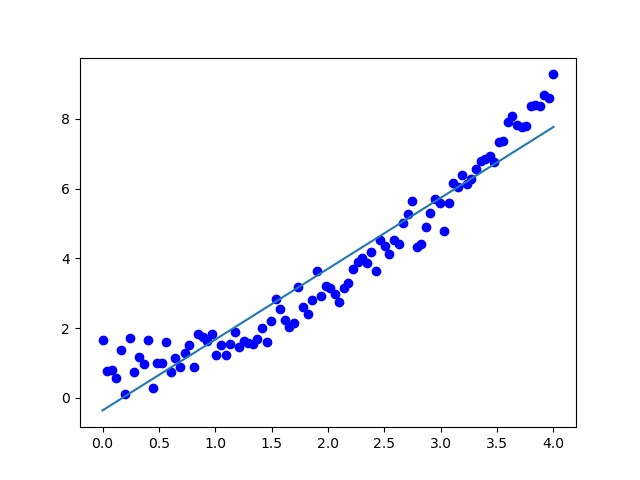
\includegraphics[scale = 0.9]{linear_normal.png}

\end{document}